\documentclass[a4paper,12pt]{article}
\usepackage{amssymb}
\usepackage{amsfonts}
\usepackage{amsthm}
\usepackage{amsmath}
\usepackage[T1]{fontenc}
\usepackage[utf8]{inputenc}
\usepackage[british]{babel}
\usepackage{times}
\usepackage{anysize}
\usepackage{color}
\usepackage{listings}
\usepackage{graphicx}
\usepackage{enumerate}
\usepackage{multicol}
\usepackage{float}

\usepackage{lmodern}  % for bold teletype font
\usepackage{xcolor}   % for \textcolor
%\lstloadlanguages{matlab}
\lstset{
	basicstyle=\ttfamily,
	columns=fullflexible,
%	frame=single,
	breaklines=true,
	postbreak=\mbox{\textcolor{red}{$\hookrightarrow$}\space},
}

\begin{document}
\begin{titlepage}
\center
\vspace*{\fill}
\Huge{Modeling of Physical Systems}\\
\Large{Radiation balance of the Earth}\\
\vspace*{1.5cm}
Dominik Katszer\\
\large{19 April 2018}
\vspace*{1.5cm}
\vspace*{\fill}
\end{titlepage}
\section{Aim of laboratory}
The aim of the laboratory is to simulate of the global radiation budget of the Earth considering two cases:
\begin{itemize}
\item assuming there is no atmosphere
\item assuming there is atmosphere
\end{itemize}
What is more, in this laboratory we were supposed to impement glaciations mechanism (Surface albedo depends on the temperature).
\section{Algorithm}
Algorithm is basing on set of energy balance equestions. In every scenario we are solving equastion in order to find temperature for specific solar constant.
\subsection{No Atmosphere}
Equastion to solve for case without atmosphere is following:
\begin{align*}
P_{Sł} =& S * \frac{Pow_z}{4} * ( 1 - A) \\
P_Z =& \sigma * T^4 * Pow_z \\
P_Z =& P_{Sł}
\end{align*}
where:
\begin{description}
\item $P_{Sł}$ -- Power of solar radiation arriving to the Earth (short wave radiation)
\item $P_{Z}$ -- Power of radiation emitted from Earth (long wave radiation)
\item $A$ -- mean albedo of the Earth surface 
\item $S$ -- solar constant
\item $Pow_{Z}$ -- area of the surface of Earth
\item $\sigma$ -- Stefan-Boltzmann constant
\item $T$ -- wanted value
\end{description}
\subsection{With Atmosphere}
\centerline{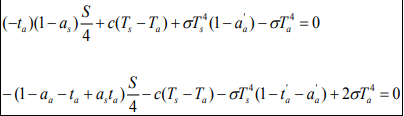
\includegraphics[scale=1]{eq}}
where:
\begin{description}
\item $ta$ – transmission of the atmosphere for short wave radiation
\item $aa$ – albedo of the atmosphere for short wave radiation
\item $as$ - surface albedo for short wave radiation
\item $ta’$- transmission of the atmosphere for long wave radiation
\item $aa’$ - albedo of the atmosphere for long wave radiation
\item $Ta$ - mean temperature of the atmosphere
\item $Ts$ - mean Surface temperature
\end{description}
In this case we are looking for $Ta$ and $Ts$. In order to observe glacier effect we change albedo of Earth surface to eqaul of ice when temperature is below $-5^\circ C$.
\section{Results}
\subsection{No Atmosphere}
Corelation between solar constant and mean temperature is presented in the figure below.
\centerline{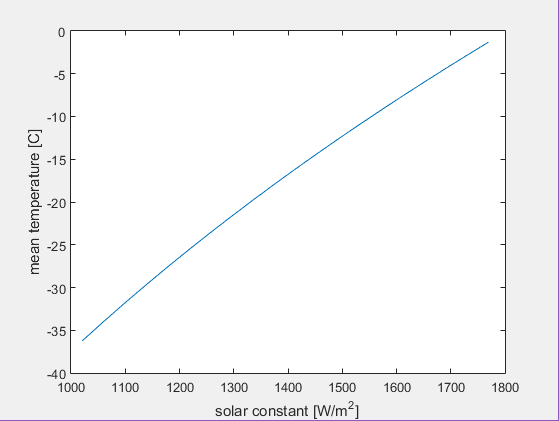
\includegraphics[scale=1]{fig1}}
\subsection{With Atmosphere}
In the following figure, glacier effect and changes of mean temperature are presented. It is worth to notice that there is a difference depending on a way how solar constant is changing (increments or decreases).\\
\centerline{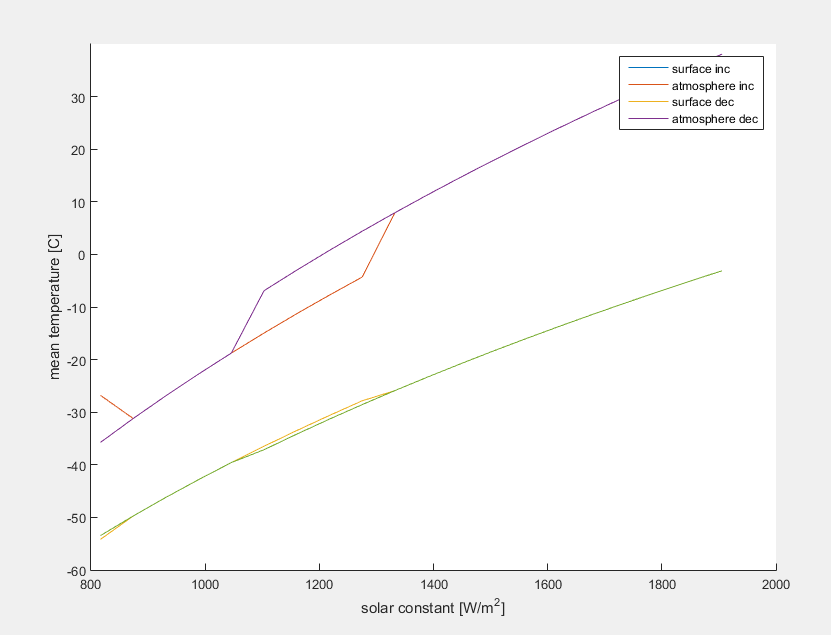
\includegraphics[scale=0.7]{fig2}}
\section{Conclusions}
This laboratory clearly shows how atmosphere have big influence on the temperature on the surface of Earth. What is more temperature is proportional to solar constant and depends on many factors, for example albedo of surface. 
\section{Source code}
Code contains some parts which were extracted int oanother files in order to achieve better readability. \\
\lstinputlisting{radiationBalance.m}
\lstinputlisting{meanTempWithAtmosphere.m}
\lstinputlisting{meanTempNoAtmosphere.m} 

\end{document}